\documentclass{article}
\usepackage[utf8]{inputenc}
\usepackage{amsmath,amssymb}
\usepackage{amsfonts}
\usepackage{paralist}
\usepackage{color}
\usepackage[table]{xcolor}
\usepackage{graphicx}
\usepackage[detect-weight=true, binary-units=true]{siunitx}
\usepackage{pgfplots}
\usepackage{authblk}
\usepackage{url}
\usepackage{multirow}
\usepackage{booktabs}
\usepackage{blindtext}
\usepackage{adjustbox}
\usepackage{subcaption}
\usepackage{float}
\usepackage[font=small, labelfont=bf, textfont=it, format=hang]{caption}
\usepackage[colorlinks=true, allcolors=blue]{hyperref}
\urlstyle{same}
\usepackage[english,nameinlink]{cleveref}
\usepackage{natbib} 
\crefname{equation}{}{}

\newcommand{\flearn}{f'_{\rm learn}}
\newcommand{\nmin}{n_{\rm min}}
\newcommand{\ntree}{n_{\rm tree}}
\title{Introduction to Machine Learning project:\\X food popularity}
\author[*]{Alessio Gaia, Carpenè Sara, Fantuzzi Giulio, Valentinis Alessio}
%\author[2]{Carpenè Sara}
%\author[3]{Fantuzzi Giulio}
%\author[4]{Valentinis Alessio}
\affil[*]{
    problem statement,
    solution design,
    solution development,
    data gathering,
    writing
}
\date{Course of AY $2023$-$2024$ - Data Science and Artificial Intelligence}

\begin{document}

\maketitle

\section{Problem statement}
\label{sec:problem_statement}
This project aims to design and develop a Machine Learning system to predict \textit{how popular} a tweet about food will be. Let $X=\{x \mid x \text{ is a tweet about food}\}$ be the set of tweets of interest. Since $x \in X$ cannot be processed directly by the machine, we first apply a pre-processing function $f_{\rm pre-proc}: X \rightarrow X'$ into a machine-interpretable space $X'$ (see \cref{ss:pre-processing}). Then, we seek to learn a model $m \in M$ from an $f'_{\rm learn}: P^{*}(X' \times Y) \rightarrow M$ and use it into an $f'_{\rm predict}: X' \times M \rightarrow Y$ to predict the output variable $y$ for an input tweet.


%Formally, given the sets $X=\{x \mid x \text{ is a tweet about food}\}$ and $Y=\mathbb{R}$, our goal is to learn a model $m \in M$ from an $f'_{learn}: P^{*}(X' \times Y) \rightarrow M$ and use it into an $f'_{predict}: X' \times M \rightarrow Y$ to predict the output variable $y$ for an input tweet.\\[0.2cm]
% Remember that we define
% \begin{align*}
% \begin{gathered}
% 	f'_{learn}: P^{*}(X' \times Y) \rightarrow M\\
% 	f'_{predict} : X' \times M \rightarrow Y.
% \end{gathered}
% \end{align*}
%\textbf{Note:} $x \in X$, being a tweet, is not directly processable by a machine, and a pre-processing phase $f_{pre-proc}: X \rightarrow X'$ is indeed required (see \Cref{ss:pre-processing}).\\[0.2cm]
% A solution based on a Machine Learning approach is suitable for this assignment: building an $f'_{learn}$ cannot be done by humans, given the nature of the problem (concerning above all complexity of the solution and human cost in dealing with thousands of observation, each with many covariates).
% Furthermore, due to what described above, the model $m \in M$ will not be simple, so performing the prediction in a computer is the only suitable choice. Given the nature of the problem we opted for a regression approach and, given also the nature of $X$ and $Y$, we opted for supervised learning techniques.
Constructing such an $\flearn$ would be too complex for humans, due to the intricate nature of the problem and the substantial human resources required to handle a multitude of observations, each with lots of details. Moreover, the complexity of the solution dictates that the model $m \in M$ will not be straightforward, so relying on computational methods is the most practical approach for the prediction phase. A Machine Learning solution is hence well-suited for the task at hand. More precisely, we will opt for a regression approach and, considering the nature of both $X$ and $Y$, supervised learning techniques emerge as the most fitting choice.

\section{Data}
\label{sec:data}
%The dataset on which to conduct our analysis was not provided, so we were required to build one.
\subsection{Web scraping}
% The dataset on which to conduct our analysis was not provided, so we were required to build one. We are not going into details of the data-gathering process; to maximaly summarize, we used the Python library \textit{ntscraper} (insert link to reference to documentation), as it allowed us to break through X's new limitation on 1500 downloadable Tweets per month, which could have resulted in too few data. Despite this, due to the computational time of the library, especially when gathering user's information, we collected a total of $4075$ tweets, written in English, containing either the word or the hashtag \textit{`food`}.
%The dataset for our analysis was not provided, necessitating the construction of one. Instead of referring to X's official APIs, the entire data-gathering process was based on the Python library \textit{ntscraper} \cite{ntsraper}. 
As no dataset was provided, we performed our analysis on data gathered using the Python library \texttt{ntscraper} \cite{ntsraper}. This library bypasses the limit to 1500 tweet downloads per month imposed by X's API, which could make our dataset insufficiently large and not representative.
%the risk of insufficient data, both in terms of size and representativeness. 
%Such a decision was primarily made to address X's new limitation of 1500 downloadable Tweets per month, which could heighten the risk of insufficient data, both in terms of size and representativeness.
%Despite the computational time constraints of the library, especially in gathering user information, 
Thanks to this library, we successfully collected a total of $4075$ English-language tweets containing either the word or the hashtag \textit{`food'}.
\subsection{Pre-processing}\label{ss:pre-processing} 
% Each observation contains some information about the tweet: text, quotes, is.retweet, external.link, pictures, videos, gifs, multimedial.content and some information about the user: user.image, user.bio, user.website, user.tweets, user.following, user.media.
% Among this variables the numerical ones are: quotes, user.tweets, user.following, user.media and the boolean ones are: is.retweet, external.link, pictures, videos, gifs, multimedial.content, user.image, user.bio, user.website.
% \noindent We implemeted some customed functions to get the number of hashtags and emojis of each text, and we added them as features. We performed pre-precessing on the text of tweets (conversion to lowercase, removal of punctuation, stemming, removal of stop words). Then we applied tf-idf vectorization of the preprocessed text, since it weight the importance of a word relative to the frequence across all the corpus. (penalizing common words and enhancing less common and more informative words.)
While the input variable is inherently digital, it is not directly processable by machines. Therefore, a pre-processing phase involving feature engineering was a key step to include in the design of our ML system.
The library \texttt{ntscraper} used for data retrieval facilitates the process, as it not only captures the text of the tweets, but also extracts features including likes, comments and retweets count, quotes, retweet status, external links, pictures, videos and gifs. The library provides also functionalities to get user details, such as profile image, bio, website and total of tweet, media, followers and following count. In a subsequent data preparation phase, a vast majority of the variables was converted into a suitable format (e.g., from \textit{string} to \textit{bool}), and some custom functions has been implemented to get additional information from texts, such as the number of hashtags and emojis in each tweet. Finally, after some basic manipulations to texts (\textit{conversion to lowercase, removal of punctuation, stemming, removal of stop words}), we performed a \textit{tf-idf} vectorization in order to penalize frequently occurring words while highlighting less common and more informative ones, contributing to the model's focus on meaningful features.

% More precisely, we kept only the words in at least 40 tweets (1\% of total tweets).
% Regarding the response variable, we opted for the engagement rate, i.e. a measure that keeps count of interaction (likes, comments, retweets) a post receive, over the total number of follower of the account that have published the tweet. In addition we applied a logarithmic transformation, to mitigate the resulting excessive skewness of this variable.
% Formally, we used as output variable the quantity $$y^{(i)} = \ln \left( \frac{1+retweets^{(i)}+likes^{(i)}+comments^{(i)}}{1+followers^{(i)}} \right)$$
% The quantity $1$ added both at numerator and denominator is applied in order not to obtain $-\infty$ or $\infty$ as values.
Regarding the response variable, we opted for a slightly different version of the \textit{engagement rate} \cite{eng-rate1, eng-rate2}, a metric that measures the overall interactions received by a tweet, divided by the total number of user's followers. Formally:
\begin{equation}\label{eq:eng-rate}
  y^{(i)} = \ln \left( \frac{x_{\rm likes}^{(i)}+x_{\rm retweets}^{(i)}+x_{\rm comments}^{(i)}+1}{x_{\rm followers}^{(i)}+1} \right)  
\end{equation}

\noindent The log transformation was applied to mitigate the skewness of the engagement, while $1$ was added both to numerator and denominator in order to extend its applicability to any tweet (avoiding also the risk to obtain infinite values).\\[0.1cm]
\textbf{Note:} once computed the engagement rate, the features involved in \Cref{eq:eng-rate} were dropped from the dataset, in order to avoid the estimation of any trivial model.

\section{Assessment and performance indexes}
\label{sec:assessment_performance_index}
% Recalling that we are dealing with a numerical and continuous output variable $Y$, it's natural to come up with measure like Root Mean Squared Error (RMSE) to assess the techniques \textit{effectiveness}.
% To deal with \textit{efficiency}, instead, we opted to evaluate the execution time of both learning and prediction phase. Times will be measured on the prediction and learning phase of the 10-fold Cross Validation used for assessing the effectiveness of the models.
To assess the degree to which our solutions solved the regression problem, we focused both on their \textit{effectiveness} and \textit{efficiency}. Effectiveness was measured by evaluating the \textit{RMSE} (the lower, the better), while efficiency was measured in terms of CPU time (in seconds), during both the learning and the prediction phase. To reach a more general and robust result, the entire procedure was based on a 10 fold cross-validation.

\section{Proposed solution}
\label{sec:solution}
% After having retrieved the data, we tested five different learning techniques, namely: (i) Dummy regressor, (ii) Regression tree, (iii) Random Forest, (iv) Support Vector Machines, (v) k-Nearest Neighbor.
We implemented different supervised learning techniques, namely: Regression Tree, Random Forest, Support Vector Regressor (SVR) and kNN. To assess their performances, we referred to the Dummy Regressor as a comparison baseline.
\subsection{Hyperparameter tuning}
% We performed 10-fold CV for hyperparameter tuning to compare these different learning techniques, in order to assess in a robust way their effectiveness.\\[0.1cm]
For each learning technique, we conducted a hyperparameter tuning phase through grid search, based on RMSE and performed within a 10-fold CV.\\[0.1cm]
\noindent
\textbf{Regression Tree} \\[0.1cm]
% The parameter tuned is $n_{\text{min}}$, the values considered are: 1, 10, 15, 25, 30, 50, 100, 150, 200, 500. The one that minimizes the RMSE is 100.\\[0.1cm]
The optimal value for $\nmin$ was found to be $\nmin=100$ after tuning across the grid $\{1, 10, 15, 25, 30, 50, 100, 150, 200, 500\}$.\\[0.2cm]
\noindent
\textbf{Support Vector Regression (SVR)}\\[0.1cm]
% First, the parameter tuned is the kernel and we consider: linear, polynomial and gaussian. The best one results the gaussian one.\\
% For each of them we consider some other parameters. The parameter tuned for the linear one is $C$ that is a regularization parameter. The values considered are 0.001,0.003,0.005,0.01,0.03,0.05. The one that minimize the RMSE is.
% The parameter tuned for the polynomial one are $C$ and the degree. The values considered are respectively: 0.001,0.005,0.03,0.05,0.1 and 2, 3, 4, 5, 6, 7. The combination that minimize the RMSE is $C$ = 0.1, degree = 2.
% The parameter tuned for the gaussian one are $C$ and the gamma (COSA é GAMMA). The values considered are respectively: 0.1,0.5,1,1.5,5,10,15,25 and scale,auto. The combination that minimize the RMSE is $C$ = 5, gamma = scale.\\[0.1cm]
% A preliminary tuning was made just on the type of kernel (among \textit{\{linear,poly,rbf\}}), and \textit{rbf} resulted the optimal one. Then, for each of them, we performed a tuning on some parameters related to the specific kernel type:\\[0.1cm]
\textbf{Linear:} the optimal value for the regularization parameter $C$ was found to be $C=0.005$ after tuning across the grid $\{0.001,0.003,0.005,0.01,0.03,0.05\}$;\\[0.15cm]
\textbf{Poly:} $C$ was tuned across the grid $\{0.001,0.003,0.005,0.01,0.03,0.05\}$, while the degree of the polynomial was tuned across the grid $\{2, 3, 4, 5, 6, 7\}$.\\
The optimal combination resulted $(C=0.1,d=2)$;\\[0.15cm]
\textbf{Rbf:} $C$ was tuned across the grid $\{0.1,0.5,1,1.5,5,10,15,25\}$, while the parameter $\gamma$ was tuned just across the default values provided by \textit{scikit-learn} \cite{scikit-learn}.\\The optimal combination resulted $(C=5,\gamma=\text{`scale'})$.\\[0.2cm]
\noindent
\textbf{k-Nearest Neighbor (kNN)} \\[0.1cm]
The optimal value for the parameter $n_{\rm neighbors}$ was found to be $n_{\rm neighbors}=20$ after tuning across the grid $\{1, 2, 5, 10, 15, 20, 50, 100\}$.
\begin{figure}[H]
  \begin{minipage}{0.33\textwidth}
    \centering
    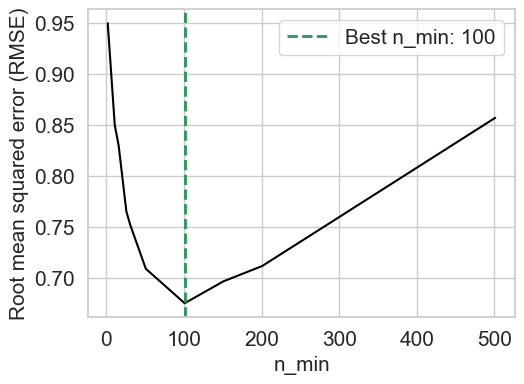
\includegraphics[scale=0.3]{rt_grid_search.png}
    \subcaption{\footnotesize Regression Tree}
    \label{fig:img1}
  \end{minipage}
  \begin{minipage}{0.33\textwidth}
    \centering
    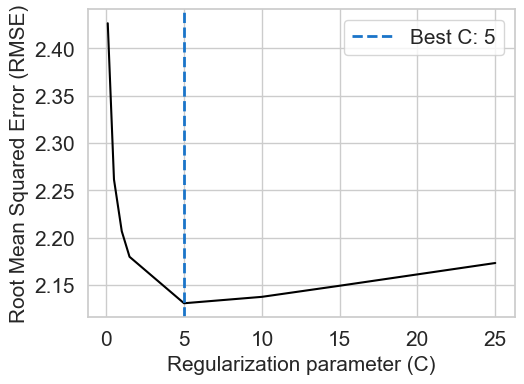
\includegraphics[scale=0.3]{svr_rbf_grid_search.png}
    \subcaption{SVR (rbf)}
    \label{fig:img3}
  \end{minipage}
  \begin{minipage}{0.32\textwidth}
    \centering
    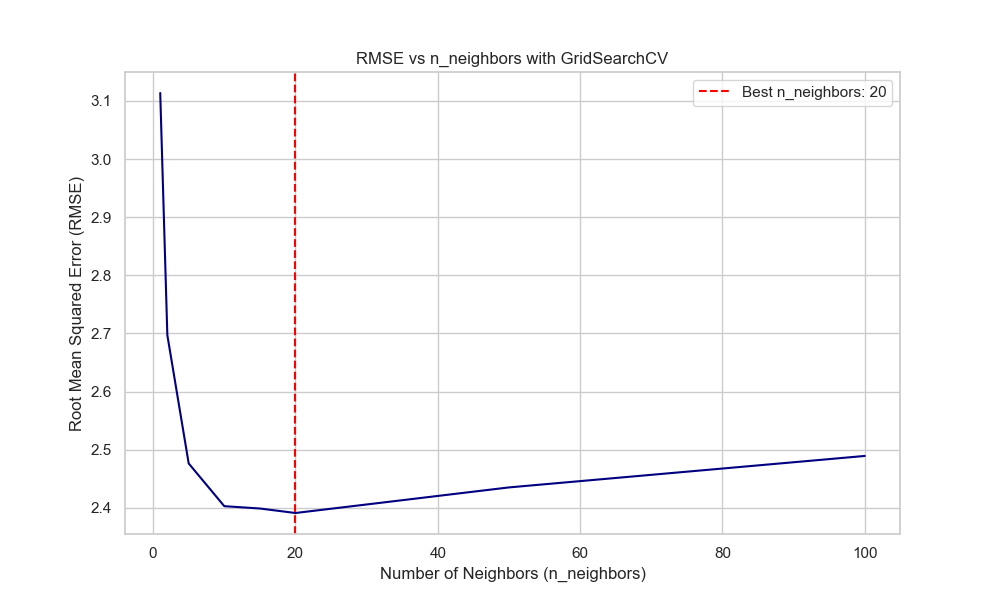
\includegraphics[scale=0.3]{knn_grid_search.png}
    \subcaption{\footnotesize kNN}
    \label{fig:img4}
  \end{minipage}
\end{figure}
\noindent
\begin{minipage}{0.55\textwidth}
    \textbf{Random Forest} \\
    Despite the parameters of such technique have good default values $\nmin=1$ and $\ntree=500$, they were still tuned across the grids $\{10, 15, 25, 50, 75, 100, 250, 500\}$ and $\{1, 10, 25, 50, 75, 100\}$. The optimal combination resulted $(\ntree = 500,\nmin = 1)$.
\end{minipage}
\begin{minipage}{0.45\textwidth}
    \centering
    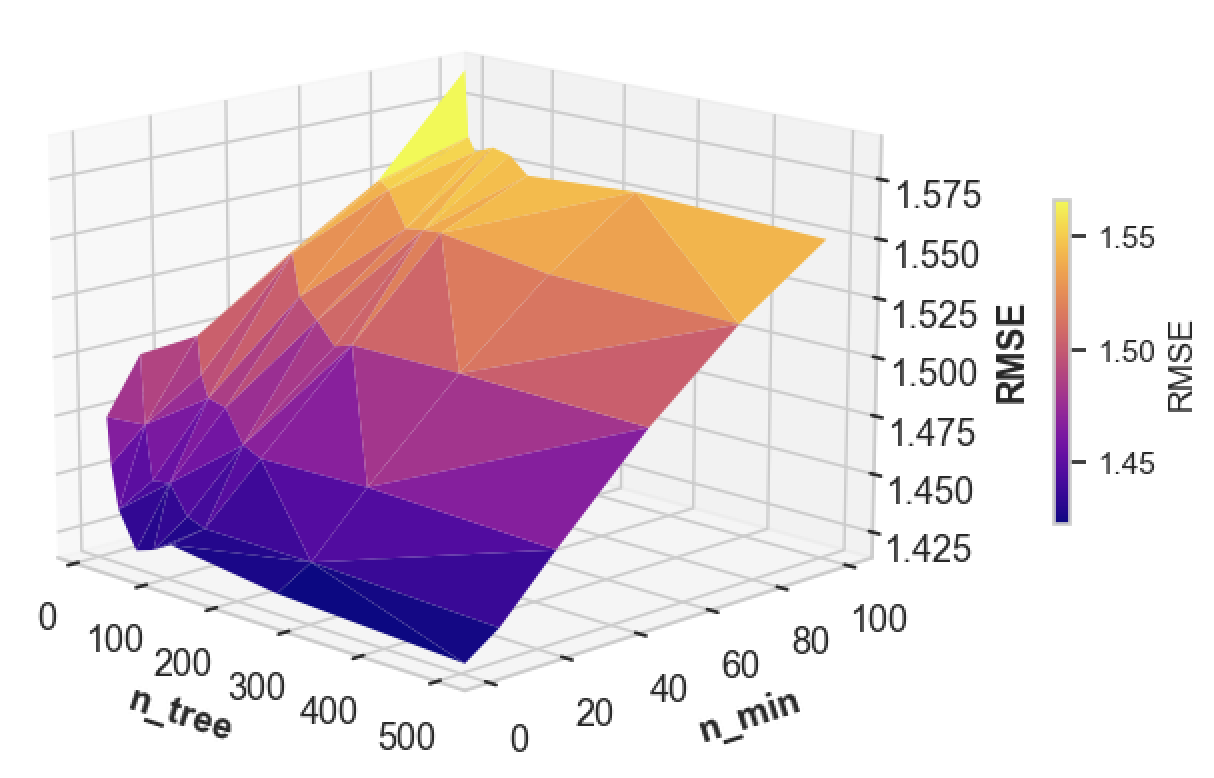
\includegraphics[scale=0.24]{rmse_vs_n_estimators_and_min_samples_split_SURFACE.png}
\end{minipage}

\section{Results and discussion}


\begin{table}
\centering
\caption{\footnotesize Performance metrics for the analyzed learning techniques}
\label{results-table}
\begin{adjustbox}{max width=\textwidth}
\begin{tabular}{l|cc|cccc|}
&\multicolumn{2}{>{\columncolor{blue!50}}c|}{\textbf{Effectiveness (RMSE)}} & \multicolumn{4}{>{\columncolor{blue!50}}c|}{\textbf{Efficiency (Time in seconds)}}\\
\hline
\multicolumn{1}{>{\columncolor{blue!50}}c|} {\textbf{Models}} & \multicolumn{1}{>{\columncolor{blue!30}}c} {$\mu$} & \multicolumn{1}{>{\columncolor{blue!30}}c|}{$\sigma$}& \multicolumn{1}{>{\columncolor{blue!30}}c}{$learn_{\mu}$}& \multicolumn{1}{>{\columncolor{blue!30}}c}{$learn_{\sigma}$}& \multicolumn{1}{>{\columncolor{blue!30}}c}{$pred_{\mu}$}& \multicolumn{1}{>{\columncolor{blue!30}}c|}{$pred_{\sigma}$} \\ 
\hline
\rowcolor{gray!10} Dummy regressor &2.549105&0.089576&0.001508&0.001075&0.000287&0.000083 \\ 
\rowcolor{white} SVR (kernel=\textit{linear})&2.226802&0.081544&1.528836&0.007922&0.156785&0.000370\\
\rowcolor{gray!10} SVR (kernel=\textit{poly})&2.414326&0.077510&1.497258&0.003428&0.159443&0.000456\\
\rowcolor{white} SVR (kernel=\textit{rbf})&2.092663&0.076907&1.650402&0.010091&0.275482&0.002714\\
\rowcolor{gray!10} kNN ($n_{\rm neighbors}=20$)&2.360611&0.067055&0.005344&0.001519&0.012011&0.002559\\
\rowcolor{white} Regression Tree ($\nmin=100$)&1.631314&0.058482&0.026548&0.005597&0.001133&0.000201\\ 
\rowcolor{gray!10} RF ($\ntree=500;\nmin=1$)&1.378885&0.054963&1.052611&0.012792&0.029593&0.004383\\
\rowcolor{gray!10} RF ($\ntree=100;\nmin=1$)&1.381328&0.057168&0.225316&0.008992&0.007599&0.000237\\
\rowcolor{white} RF ($\ntree=100;\nmin=20$)&1.408994&0.051836&0.159062&0.005354&0.007049&0.000198\\
\hline
\end{tabular}
\end{adjustbox}
\label{res_table}
\end{table}
% \end{adjustbox}\\[0.5cm]

% \noindent
% The table above highlights that by using the optimized parameters the Random Forest technique emerges as the best
% technique to tackle the problem, as indicated by the lower Root Mean Squared Error (RMSE). \\
% \noindent
% Obviously the most efficient method result to be the Dummy classifier, as we could imagine, but it is the most ineffective by far.\\
% On the contrary, it's interesting to observe that in our analysis, Support Vector Regression (SVR) performs poorly in both the learning and prediction phases, and it results in one of the worst techniques.\\
% \noindent
% An interesting aspect to explore is how the trade-off between effectiveness and efficiency evolves by relaxing certain hyperparameters of Random Forest (and Trees).
% INSERIRE ANALISI CON PARAMETRI NON OTTIMALI E VEDERE TEMPI ED ERRORE.\\
% \noindent
% One of the first aspects in which this analysis would get better is try and gather more data, which would result in a better and more precise learning phase. In fact, such a small data set may not be fully representative of the system.
% With a larger dataset, tit would be interesting to perform again some hyperparameter tuning, determining whether the observed hierarchy of techniques holds or if certain methods gain effectiveness.\\
% In conclusion, expanding the dataset would enable a more robust and precise learning phase, potentially leading to further insights and improvements in the overall model performance.

% GIULIO
Results of our computational experiments are illustrated in \cref{results-table,res-fig}.
The Dummy regressor, though highly efficient, demonstrates limited predictive capability and, as expected, it resulted in the worst learning technique (highest \textit{RMSE}). Surprisingly, despite its greater inner complexity, SVR ranks among the least effective techniques, requiring the longest time for both learning and prediction. In contrast, Regression Tree shows improved effectiveness, with an RMSE  approximately $36\%$ better than the Dummy regressor and $22\%$ better than SVR with a Gaussian kernel (the most effective SVR configuration). While not as efficient as the Dummy regressor, it balances predictive capability with computational efficiency. As for kNN, it falls between Regression Tree and SVR in terms of effectiveness, and is efficient in learning but slower in prediction (approximately 26 times slower than Tree). Finally, to showcase the \textit{`Wisdom of the trees'} principle, Random Forest with $\ntree=500$ and $\nmin=1$ outperforms Regression Trees and boasts the lowest \textit{RMSE}, emerging as the most effective technique analyzed. However, its moderately efficiency comes at the cost of relatively slower predictions. Exploring relaxed hyperparameter values reveals a subtle interplay between predictive accuracy and computational efficiency. For instance, with $\nmin=20$ and $\ntree=100$ the \textit{RMSE} grows by only $2.14\%$, while learning and prediction are as much as $84.89\%$ and $76.18\%$ faster, respectively.
\begin{figure}[h]
    \centering
    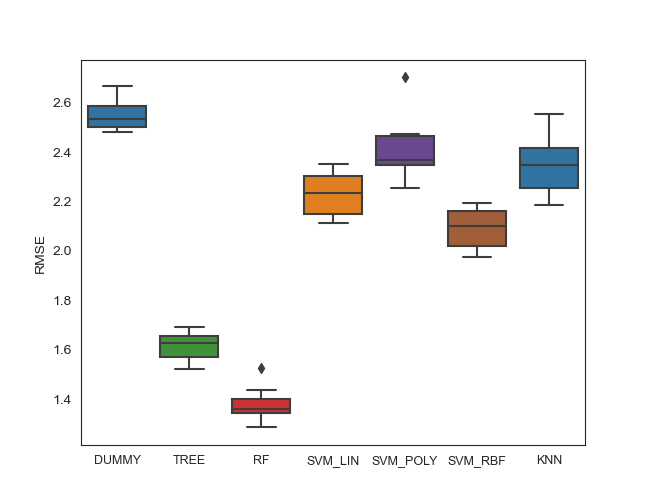
\includegraphics[width=0.8\textwidth]{techniques_comparison_rmse.png}
    \caption{\footnotesize Boxplot of learning techniques with optimal hyperparameters}
    \label{res-fig}
\end{figure}
% One of the first aspects in which this analysis would get better is try and gather more data, which would result in a better and more precise learning phase. In fact, such a small data set may not be fully representative of the system. With a larger dataset, tit would be interesting to perform again some hyperparameter tuning, determining whether the observed hierarchy of techniques holds or if certain methods gain effectiveness. In conclusion, expanding the dataset would enable a more robust and precise learning phase, potentially leading to further insights and improvements in the overall model performance
\newpage
\nocite{slides,james2013introduction}
\bibliographystyle{plain}
\bibliography{bibliography}

\end{document}
